\chapter{图的稀疏化}
\label{chap:graph-sparsification}

在前面两章的拉普拉斯方程迭代求解与谱划分中，每计算一次拉普拉斯矩阵与向量的乘积$\bm L\bm x$，都要遍历图中的所有$m$条边。当原图$\mathcal G$是边数高达$\Theta(n^2)$的稠密图时，矩阵乘法每次需要$O(n^2)$时间。如果能用一张共享同一顶点集$V$、但边数仅有$O(n\log n/\varepsilon^2)$的稀疏重加权子图$\mathcal H$来代替原图$\mathcal G$，对$\mathcal H$的矩阵乘法只需按其边数计时；能否加速原问题，还取决于近似误差、构造成本与后续算法。

然而，简单地随机删边很容易破坏图的关键结构：设两个稠密大团之间仅靠一条细桥相连，一旦删边时漏掉了这条桥，两团之间的割权会从正数降为零，图由连通变为不连通；相反，若删去的是稠密团内部的一条边，由于两端顶点之间还有大量并联替代路径，可以尝试通过保留边重加权控制误差，但仍须验证谱近似条件。

这一对比说明，构造稀疏图必须回答三个核心问题：第一，什么样的替代图$\mathcal H$才算在数学上严格逼近了原图$\mathcal G$？第二，应当按什么概率抽取原图的边、并如何重新分配权重，才能既保留关键瓶颈边又大幅削减冗余边？第三，如何利用构造出的稀疏图加速原图拉普拉斯方程的求解？

本章讨论无向无自环图，设原图$\mathcal G=(V,E,c)$包含$n=|V|\geq 2$个顶点和$m=|E|$条正权边，替代图$\mathcal H=(V,E_H,\widehat c)$保留全部顶点并从$E$中选取子集重新赋权。对每条边$e=\{u,v\}\in E$，固定任意参考方向并记边关联向量为$\bm b_e=\bm e_u-\bm e_v\in\mathbb R^n$，则顶点赋值向量$\bm x\in\mathbb R^n$在原图与替代图上的拉普拉斯二次型分别为
\[
\bm x^\top\bm L_G\bm x
=\sum_{e\in E}c_e(\bm b_e^\top\bm x)^2,
\qquad
\bm x^\top\bm L_H\bm x
=\sum_{e\in E_H}\widehat c_e(\bm b_e^\top\bm x)^2.
\]
第~\ref{sec:graph-sparsification-approximation}节首先定义割近似与谱近似，说明谱近似对线性求解所提供的额外控制，并分别证明谱近似保持特征值、有效电阻与方程解的三条核心性质；第~\ref{sec:graph-resistance-sampling}节直接调用第~\ref{sec:graph-sparsification-resistance-trees}小节的生成树包含概率与Foster定理，给出基于有效电阻抽样的稀疏图构造算法与矩阵Chernoff界证明；第~\ref{sec:graph-sparse-preconditioning}节展示如何将稀疏图作为预条件子加速原图拉普拉斯方程的共轭梯度求解。

\section{割近似与谱近似}
\label{sec:graph-sparsification-approximation}

稀疏化的目标是用一张边少得多的图来代替原图。但代替到什么程度才算够用？本节先从割权开始回答这个问题，再把要求提高到所有实值向量上的能量。

\subsection{割近似}
\label{sec:graph-cut-approximation}

假设原来某个割的权是十。如果允许百分之十的误差，替代图上这个割的权落在九和十一之间就算可以接受。如果原来的割权为零，相对误差要求替代图上也是零——两团之间没边的判断不能弄错。

但是，稀疏化是在看到任何特定的割之前就已经选定了一张替代图。之后在替代图上搜索最小割时，算法会逐一比较各种分组，其中可能恰好有一种分组的跨边被删掉了许多。因此我们要求先固定替代图，再让它对\emph{每一个}分组都满足同一个相对误差。

\begin{definition}[割近似]
\label{def:graph-cut-approximation}
设$\mathcal G$与$\mathcal H$有同一顶点集$V$，$0<\varepsilon<1$。对$S\subseteq V$，记$\overline S=V\setminus S$，用$c_G(S,\overline S)$和$c_H(S,\overline S)$分别表示两图中跨越该割的边权之和。若每个$S$都满足
\begin{equation}
(1-\varepsilon)c_G(S,\overline S)
\leq c_H(S,\overline S)
\leq (1+\varepsilon)c_G(S,\overline S),
\label{eq:graph-cut-approximation}
\end{equation}
就说$\mathcal H$是$\mathcal G$的一个$\varepsilon$\term{割近似}（cut approximation）。
\end{definition}

下界系数$1-\varepsilon$是正数，所以原图中有正权边跨越的割，在$\mathcal H$中仍有正权边跨越。零割也自动保持为零。这保证了"某一组顶点与外部是否相连"的判断不变。

\paragraph{最小割的继承}

记$C_G$和$C_H$为两图的最小割权。两图的分组候选完全相同，但取到最小值的分组可能不同。

先给$C_H$找一个下界。设$S^*_H$是$\mathcal H$中的最优分组，按割近似的上界，它在$\mathcal H$中的割权至多是它在$\mathcal G$中割权的$1+\varepsilon$倍。反过来，$\mathcal G$中的最优分组$S^*_G$作为$\mathcal H$的一个候选，其在$\mathcal H$中的割权至少是在$\mathcal G$中的$1-\varepsilon$倍。$\mathcal H$的最小割不超过任何候选，$\mathcal G$的最小割不超过$S^*_H$在$\mathcal G$上的值，因此
\begin{equation}
(1-\varepsilon)C_G\leq C_H\leq(1+\varepsilon)C_G.
\label{eq:graph-sparsification-min-cut}
\end{equation}

\paragraph{RatioCut的继承}

第~\ref{chap:spectral-partition}章的RatioCut把割权乘以$1/|S|+1/|\overline S|$。两图共享同一个顶点集，因此这个因子在每个割上完全相同。割权的$1\pm\varepsilon$比例直接传给了RatioCut的目标值，最优值也是如此。

\paragraph{体积和导通率的继承}

导通率和NCut还用到集合的\emph{体积}，即一侧顶点的加权度之和$\operatorname{vol}_G(S)=\sum_{i\in S}d_i$。换了边权后，各顶点的加权度也会改变。

取单点集合$\{v\}$。它的割恰好由$v$的所有关联边组成，因此式~\eqref{eq:graph-cut-approximation}也控制了每个顶点的加权度。将组内所有顶点的度下界相加或上界相加，得到
\begin{equation}
(1-\varepsilon)\operatorname{vol}_G(S)
\leq \operatorname{vol}_H(S)
\leq (1+\varepsilon)\operatorname{vol}_G(S).
\label{eq:graph-sparsification-volume}
\end{equation}
需要注意的是，组内边在组内两个顶点的度里各计一次，但在$S$的割权中不出现。

第~\ref{sec:graph-cheeger}节的导通率以割权为分子、以较小一侧的体积为分母。分子和分母都可能偏离原值。用割权下界除以体积上界，可以得到导通率的下界；用割权上界除以体积下界，得到上界。记两图的导通率为$\phi_G(S)$和$\phi_H(S)$，整理后
\begin{equation}
\frac{1-\varepsilon}{1+\varepsilon}\phi_G(S)
\leq \phi_H(S)
\leq \frac{1+\varepsilon}{1-\varepsilon}\phi_G(S).
\label{eq:graph-sparsification-conductance}
\end{equation}
NCut是割权分别除以两侧体积之后的和。每一项都继承同样的比例界，两图的正体积集合相同，因此可以在相同的合法划分上取最小来比较最优值。

\subsection{谱近似}
\label{sec:graph-spectral-approximation}

割近似只看指示向量——每个顶点要么在$S$中取一、要么在$\overline S$中取零。这时跨割边两端的差平方都是一，能量就等于跨割的边权之和。

但谱划分的松弛和拉普拉斯方程用到的是\emph{任意实值}的顶点赋值。两端相差五的那条边和两端相差零点一的那条边，对能量的贡献可以差几个数量级。单纯比较跨边总权看不出重加权集中在差异大的边还是差异小的边。因此需要一种更严格的保证：让替代图在\emph{每一种}赋值上的能量都接近原图。

\begin{definition}[谱近似]
\label{def:graph-spectral-approximation}
设$\bm L_G$和$\bm L_H$是同一顶点集上两图的拉普拉斯矩阵。若对每个$\bm x\in\mathbb R^n$都有
\begin{equation}
(1-\varepsilon)\bm x^\top\bm L_G\bm x
\leq \bm x^\top\bm L_H\bm x
\leq (1+\varepsilon)\bm x^\top\bm L_G\bm x,
\label{eq:graph-spectral-approximation-energy}
\end{equation}
则称$\mathcal H$是$\mathcal G$的一个$\varepsilon$\term{谱近似}（spectral approximation）。用半正定序写，就是
\begin{equation}
(1-\varepsilon)\bm L_G\preceq\bm L_H\preceq(1+\varepsilon)\bm L_G.
\label{eq:graph-spectral-approximation-order}
\end{equation}
边数显著减少且满足此条件的构造称为\term{谱稀疏化}（spectral sparsification）。
\end{definition}

谱近似蕴含割近似。只需在式~\eqref{eq:graph-spectral-approximation-energy}中把$\bm x$取成子集$S$的指示向量——只有跨割边的两端值不同，差的平方都是一，因此能量恰好等于割权。代入后就得到式~\eqref{eq:graph-cut-approximation}。

谱近似还自动保留连通分量。若$\bm x^\top\bm L_G\bm x=0$，上界迫使$\bm x^\top\bm L_H\bm x=0$。反过来，若$\bm x^\top\bm L_H\bm x=0$，正的下界系数$1-\varepsilon$迫使原图能量也为零。第~\ref{sec:graph-laplacian-kernel}节说过，能量为零要求在每个正权连通分量上取常值。因此两图的零能量方向完全相同，连通分量也完全相同。

对连通图，只有常值方向的能量为零。在$\bm 1^\perp$中，非零向量的能量为正，可以取拉普拉斯的逆。

\paragraph{割近似不蕴含谱近似}

反过来的推论不成立。下面用一个三顶点的例子说明，满足割近似的替代图在某个实值向量上的能量可以超出谱近似的允许范围。

\begin{example}[满足割界的图可以超出同一谱界]
\label{ex:graph-cut-not-spectral}
令$\mathcal G$是单位权三角形，三条边的权都是一。取$0<\varepsilon<1/2$，构造替代图$\mathcal H$：把边$12$的权增加$2\varepsilon$，把边$23$的权减少$2\varepsilon$，边$13$保持不变，
\[
c_H(12)=1+2\varepsilon,\qquad c_H(23)=1-2\varepsilon,\qquad c_H(13)=1.
\]

先检查割近似。原图中每个顶点都连着两条单位权边，三个单点割的权都是二。替代图中：顶点$1$的两条边权之和为$(1+2\varepsilon)+1=2+2\varepsilon$，顶点$2$的为$(1+2\varepsilon)+(1-2\varepsilon)=2$，顶点$3$的为$(1-2\varepsilon)+1=2-2\varepsilon$。三个数都落在$2(1\pm\varepsilon)$之间。因为两点割和它的单点补割权相同，所以全部六个非平凡割都满足式~\eqref{eq:graph-cut-approximation}。

再取顶点赋值$\bm x=(3,-2,-1)^\top$。三条边上两端差的平方分别是
\[
(3-(-2))^2=25,\qquad ((-2)-(-1))^2=1,\qquad (3-(-1))^2=16.
\]
原图能量为$25+1+16=42$。替代图的能量为
\[
25(1+2\varepsilon)+1\cdot(1-2\varepsilon)+16\cdot1=42+48\varepsilon.
\]
比如取$\varepsilon=1/4$。此时所有割权都在原值的$75\%$到$125\%$之间——割近似完全满足。但这个向量的能量从$42$升到了$54$，超过了谱近似允许的上界$42\times 5/4=52.5$。

能量比为$1+48\varepsilon/42=1+8\varepsilon/7$，严格大于$1+\varepsilon$。原因在于：顶点$2$的单点割看到的两条边权一增一减，总和不变。但这个实值赋值在边$12$上的差平方为$25$，在边$23$上只有$1$，增权集中在能量高的边上，减权集中在能量低的边上，二者无法对消。图~\ref{fig:sparsification-cut-energy}并排画出两图和同一个赋值，便于逐边比较。
\end{example}

\begin{BookInlineFigure}
  \centering
  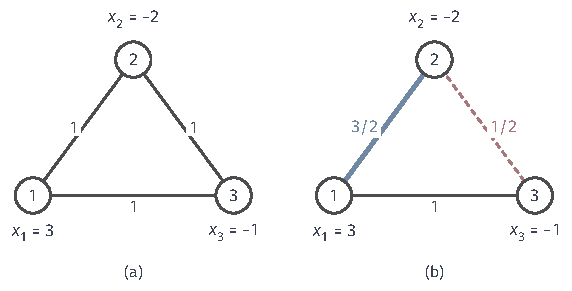
\includegraphics{figures/03-graphs/05-matrices-and-spectra/tikz/sparsification-cut-energy/figure.pdf}
  \caption{单位权原图（a）和取$\varepsilon=1/4$的替代图（b）。粗实线表示增重的边，虚线表示减重的边。三个单点割的权都满足$1\pm\varepsilon$比例，但按相同的顶点赋值$(3,-2,-1)$计算能量，替代图从$42$升到$54$，超出了谱近似的允许范围。}
  \label{fig:sparsification-cut-energy}
\end{BookInlineFigure}


\subsection{谱近似保持的量}
\label{sec:graph-spectral-approximation-consequences}

有了谱近似图，可以用它来估计原图的特征值、有效电阻和方程解。这三种比较共用同一个能量界，但各自控制的量不同：特征值来自能量商的极值，后两种还需要把比较从拉普拉斯传到逆矩阵上。

\paragraph{特征值的保持}

先把两图的组合拉普拉斯特征值各按从小到大排序。对每个$i$，想要比较第$i$个特征值。

式~\eqref{eq:graph-spectral-approximation-energy}对每个非零向量成立，两边同除以$\bm x^\top\bm x$仍然成立。左边和右边变成了Rayleigh商的比例界。在同一个$i$维子空间上分别对两图取商的最大值，原来的比例界不变。再在所有$i$维子空间中取最小值——Courant--Fischer原理（可参考\BookChapterRef{chap:condition-and-spectral-perturbation}{卷二"条件数与谱扰动"章}）说这个极值就是第$i$个特征值。因此
\begin{equation}
(1-\varepsilon)\lambda_i(\bm L_G)
\leq \lambda_i(\bm L_H)
\leq (1+\varepsilon)\lambda_i(\bm L_G).
\label{eq:graph-sparsification-eigenvalue}
\end{equation}
这只比较排序后的谱值。逐个特征向量或子空间的稳定性需要额外分析，特别是在特征值接近时。

\paragraph{有效电阻的保持}

有效电阻用到拉普拉斯的逆。为了把能量的正向比较变成逆矩阵的比较，先换一套坐标，让原图变成单位矩阵。

设原图连通，在$\bm 1^\perp$上操作。令$\bm y=\bm L_G^{1/2}\bm x$，原图能量就是$\lVert\bm y\rVert_2^2$。将$\bm x=\bm L_G^{-1/2}\bm y$代入替代图的能量，得到$\bm y^\top\bm A\bm y$，其中
\[
\bm A=\bm L_G^{-1/2}\bm L_H\bm L_G^{-1/2}.
\]
能量界对每个$\bm y$成立，因此
\begin{equation}
(1-\varepsilon)\bm I\preceq\bm A\preceq(1+\varepsilon)\bm I.
\label{eq:graph-sparsification-normalized-order}
\end{equation}
这意味着$\bm A$的每个特征值都落在$[1-\varepsilon,1+\varepsilon]$中。

取逆就是对同一组正交特征方向分别取倒数。$1-\varepsilon$变成$1/(1-\varepsilon)$，$1+\varepsilon$变成$1/(1+\varepsilon)$。注意取倒数会翻转大小关系——原来的下界变成了新的上界。图~\ref{fig:sparsification-inverse-band}用数轴标出这个翻转。

\begin{BookInlineFigure}
  \centering
  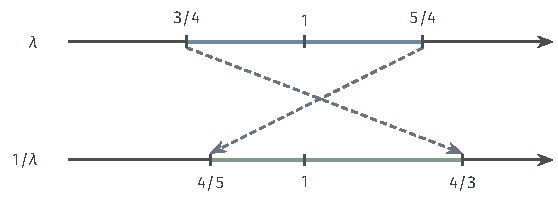
\includegraphics{figures/03-graphs/05-matrices-and-spectra/tikz/sparsification-inverse-band/figure.pdf}
  \caption{能量坐标中谱值的允许区间。虚线示意两端取倒数后怎样换位：靠左的$1-\varepsilon$变到$1/(1-\varepsilon)$一端。中间的$1$保持不动。}
  \label{fig:sparsification-inverse-band}
\end{BookInlineFigure}

将三个因子依次反向取逆，$\bm A^{-1}=\bm L_G^{1/2}\bm L_H^{-1}\bm L_G^{1/2}$。对逆矩阵的比较式两边同乘$\bm L_G^{-1/2}$，中间还原为$\bm L_H^{-1}$，上下界的单位阵还原为$\bm L_G^{-1}$。在全体向量上，两个逆都在常数方向取零，由此得到伪逆的比较
\begin{equation}
\frac{1}{1+\varepsilon}\bm L_G^\dagger
\preceq \bm L_H^\dagger
\preceq \frac{1}{1-\varepsilon}\bm L_G^\dagger.
\label{eq:graph-sparsification-inverse-order}
\end{equation}

把两点差向量$\bm e_u-\bm e_v$代入这三个二次型。按第~\ref{sec:graph-effective-resistance}节的有效电阻公式，
\begin{equation}
\frac{R_G(u,v)}{1+\varepsilon}
\leq R_H(u,v)
\leq \frac{R_G(u,v)}{1-\varepsilon}.
\label{eq:graph-sparsification-resistance}
\end{equation}
直觉上，替代图若整体提高了能量，通相同电流所需的电势差会降低——这对应了取逆之后比例关系的翻转。

\paragraph{方程解的保持}

设$\bm b\in\bm 1^\perp$，$\bm x_G=\bm L_G^\dagger\bm b$是原图的零均值解，$\bm x_H=\bm L_H^\dagger\bm b$是替代图的零均值解。我们想知道用$\bm x_H$代替$\bm x_G$会产生多大的误差。

先把两个解都放到原图的能量坐标中。令$\bm y_G=\bm L_G^{1/2}\bm x_G$，$\bm y_H=\bm L_G^{1/2}\bm x_H$。在这个坐标下，原解变成了
\[
\bm y_G=\bm L_G^{-1/2}\bm b.
\]
把$\bm x_H=\bm L_G^{-1/2}\bm y_H$代入替代图的方程$\bm L_H\bm x_H=\bm b$，两边左乘$\bm L_G^{-1/2}$，得到
\[
\bm A\bm y_H=\bm L_G^{-1/2}\bm b.
\]
右端和原解的方程相同，因此$\bm y_H=\bm A^{-1}\bm y_G$。两解的差为
\[
\bm y_H-\bm y_G=(\bm A^{-1}-\bm I)\bm y_G.
\]
在$\bm A$的正交特征基中，$\bm A^{-1}-\bm I$把每个方向乘以$1/\lambda-1$，其中$\lambda$是该方向的特征值。因为$1-\varepsilon\leq\lambda\leq1+\varepsilon$，这个乘数的绝对值至多是$\varepsilon/(1-\varepsilon)$。

按坐标定义，新坐标中的普通长度就是原图能量的平方根。因此
\begin{equation}
\lVert\bm x_H-\bm x_G\rVert_{\bm L_G}
\leq \frac{\varepsilon}{1-\varepsilon}
      \lVert\bm x_G\rVert_{\bm L_G},
\label{eq:graph-sparsification-solution-error}
\end{equation}
其中$\lVert\bm z\rVert_{\bm L_G}=\sqrt{\bm z^\top\bm L_G\bm z}$是$\bm 1^\perp$上的能量范数。这个界控制的是误差在原图上的总沿边变化，而非某个特定坐标的相对误差——如果某个坐标恰好为零，无法以它为分母给出相对界。

用于电阻查询时应读式~\eqref{eq:graph-sparsification-resistance}，用于方程近似时应读式~\eqref{eq:graph-sparsification-solution-error}，只评估划分目标时割权和体积的比较已经足够。

\section{稀疏图的构造}
\label{sec:graph-resistance-sampling}

明确了谱近似的目标后，接下来的核心问题是：\emph{如何从原图$\mathcal G$的$m$条边中只选出少量的边，构造出满足$(1-\varepsilon)\bm L_G\preceq\bm L_H\preceq(1+\varepsilon)\bm L_G$的稀疏图$\mathcal H$？}Spielman与Srivastava于2011年给出了一种随机抽样构造法：以每条边的电导与有效电阻之积$c_e R_e$作为重要性权重，从原图边集中独立有放回地抽取$q$次边，并对抽中的边按概率倒数补偿权重\scite{spielman2011graph}。本节分三步介绍抽样分布的选择、具体算法实现以及基于矩阵Chernoff界的理论证明。

\subsection{抽样分布的选择}
\label{sec:graph-resistance-sampling-distribution}

要通过随机抽边构造稀疏图，首先需要决定每条边$e\in E$在单次抽取中被选中的概率$p_e$。最朴素的想法是所有边等概率抽取（$p_e=1/m$），但它可能以很高概率漏掉维持连通性的桥边。

\paragraph{均匀抽样的风险}

考察图~\ref{fig:graph-sparsification-bridge}所示的杠铃图：左右两个稠密大团之间只有一条唯一的桥边$e_{\mathrm{bridge}}$。若在全部$m$条边中等概率独立抽样$q$次（$q\ll m$），则单次未抽中桥边的概率为$1-1/m$，连续$q$次都漏掉桥边的概率高达$(1-1/m)^q\approx\mathrm e^{-q/m}\approx 1$。

漏掉桥边会使谱近似下界不成立。为说明这一点，取一个在左团所有顶点上赋$1$、在右团所有顶点上赋$0$的测试向量$\bm x$。在左右两个团内部，每条边两端取值相同，能量贡献全为$0$；整张图在$\bm x$方向上的非零能量$\bm x^\top\bm L_G\bm x=c_{e_{\mathrm{bridge}}}>0$完全由这条桥边独自承担。漏掉桥边会使替代图在该方向上的能量变为$\bm x^\top\bm L_H\bm x=0$，直接违背谱近似要求的正下界$(1-\varepsilon)\bm x^\top\bm L_G\bm x$。

\begin{figure}[!htb]
  \centering
  \begingroup
\definecolor{SparseBridgeBlue}{HTML}{7188A3}
\definecolor{SparseBridgeBlueFill}{HTML}{E5EAF0}
\definecolor{SparseBridgeYellow}{HTML}{B4A16F}
\definecolor{SparseBridgeNeutral}{HTML}{4C4D4F}
\definecolor{SparseBridgeText}{HTML}{3B4252}
\begin{tikzpicture}[x=10mm,y=10mm,
  vertex/.style={circle,draw=SparseBridgeBlue,fill=SparseBridgeBlueFill,
    minimum size=3.2mm,inner sep=0pt,line width=.65pt},
  inneredge/.style={draw=SparseBridgeNeutral,line width=.75pt},
  bridge/.style={draw=SparseBridgeYellow,line width=1.4pt},
  text=SparseBridgeText]
  \coordinate (l1) at (0,0);
  \coordinate (l2) at (.75,.65);
  \coordinate (l3) at (1.5,0);
  \coordinate (l4) at (.75,-.65);
  \coordinate (r1) at (3.5,0);
  \coordinate (r2) at (4.25,.65);
  \coordinate (r3) at (5,0);
  \coordinate (r4) at (4.25,-.65);
  \draw[inneredge] (l1) -- (l2) -- (l3) -- (l4) -- cycle
                    (l1) -- (l3) (l2) -- (l4);
  \draw[inneredge] (r1) -- (r2) -- (r3) -- (r4) -- cycle
                    (r1) -- (r3) (r2) -- (r4);
  \draw[bridge] (l3) -- node[above,font=\footnotesize\sffamily]{桥} (r1);
  \foreach \point in {l1,l2,l3,l4,r1,r2,r3,r4}{
    \node[vertex] at (\point) {};
  }
  \node[below,font=\footnotesize] at (.75,-.87) {$x_v=1$};
  \node[below,font=\footnotesize] at (4.25,-.87) {$x_v=0$};
\end{tikzpicture}
\endgroup

  \caption{两个稠密团之间仅靠一条桥边相连。取在左团恒为$1$、右团恒为$0$的顶点函数时，两团内部边毫无能量贡献，桥边独自承担该方向的全部能量；若抽样漏掉桥边，谱近似立刻失效。}
  \label{fig:graph-sparsification-bridge}
\end{figure}

\paragraph{按有效电阻分配抽样概率}

怎样自动识别出像桥边这样决定某些方向上全部能量的边？第~\ref{sec:graph-sparsification-resistance-trees}小节建立的有效电阻与生成树理论已经给出了答案。一方面，由定理~\ref{thm:graph-tree-edge-probability}，每条边$e$的电导与有效电阻之积$c_e R_e\in(0,1]$恰好等于该边出现在随机生成树中的概率$\mathbb P(e\in T)=c_e R_e$：对于唯一的桥边，$c_e R_e=1$；而对于存在大量并联替代路径的稠密团内边，$c_e R_e$很小（如$K_n$中仅为$2/n$）。另一方面，由Foster定理（定理~\ref{thm:graph-foster-theorem}），在含$n$个顶点的连通图上，全体边的$c_e R_e$之和恒等于常数$\sum_{e\in E}c_e R_e=n-1$。

因此，将每条边的$c_e R_e$除以归一化常数$n-1$，就得到了一个合法的边抽样概率分布：
\begin{equation}
p_e=\frac{c_eR_e}{\sum_{f\in E}c_fR_f}=\frac{c_eR_e}{n-1}\qquad(e\in E).
\label{eq:graph-resistance-sampling-probability}
\end{equation}
在连通正权图（$n\geq 2$）上，每条正权边的有效电阻$R_e>0$，故$p_e>0$且$\sum_{e\in E}p_e=1$。

\paragraph{重加权补偿与单次波动界}

有了抽样概率$\{p_e\}_{e\in E}$，我们从边集中按分布$p_e$独立有放回地抽取$q$次，记第$j$次抽中的边为$e_j$（$j=1,\ldots,q$）。对于任意一条固定边$e\in E$，它在单次抽取中被选中的概率是$p_e$，$q$次抽取中平均被选中$qp_e$次。为了让它在替代图$\mathcal H$中的\emph{期望总权重}恰好等于原图权重$c_e$，规定每当边$e$被抽中一次，就给它的新权重累加$\frac{c_e}{qp_e}$（抽中概率$p_e$越小的边，一旦抽中获得的单次权重补偿越大）。将全部$q$次抽取的秩一拉普拉斯项相加，得到稀疏图$\mathcal H$的拉普拉斯矩阵：
\begin{equation}
\bm L_H
=\sum_{j=1}^q \frac{c_{e_j}}{qp_{e_j}}
     \bm b_{e_j}\bm b_{e_j}^\top.
\label{eq:graph-resistance-sampling-laplacian}
\end{equation}
沿用式~\eqref{eq:graph-sparsification-normalized-order}在正交补空间$\bm 1^\perp$上的原图能量坐标$\bm y=\bm L_G^{1/2}\bm x$，将第$j$次抽中边$e_j$所贡献的标准化秩一随机矩阵记为
\begin{equation}
\bm X_j=\frac{c_{e_j}}{qp_{e_j}}
     (\bm L_G^{-1/2}\bm b_{e_j})
     (\bm L_G^{-1/2}\bm b_{e_j})^\top.
\label{eq:graph-resistance-sampling-standardized}
\end{equation}
下面的引理揭示了有效电阻抽样分布$p_e=\frac{c_e R_e}{n-1}$如下代数性质：它不仅保证了期望无偏（$\mathbb E[\bm L_H]=\bm L_G$），而且把每一条边在最坏能量方向上的单次算子范数$\lVert\bm X_j\rVert_2$完全拉平为同一个常数$\frac{n-1}{q}$。

\begin{lemma}[有效电阻抽样的无偏性与单次范数界]
\label{lem:graph-resistance-sampling-moments}
设连通正权图按概率$p_e=c_eR_e/(n-1)$独立有放回抽取$q$次边构造式~\eqref{eq:graph-resistance-sampling-laplacian}的$\bm L_H$。则：
\begin{enumerate}
  \item 抽样矩阵的期望等于原图拉普拉斯矩阵：
  \begin{equation}
  \mathbb E[\bm L_H]=\bm L_G,\qquad
  \mathbb E\!\left[\sum_{j=1}^q\bm X_j\right]=\bm I_{\bm 1^\perp}.
  \label{eq:graph-resistance-sampling-expectation}
  \end{equation}
  \item 不论第$j$次抽中哪一条边$e_j\in E$，标准化单次矩阵$\bm X_j$都是对称半正定的，且其算子谱范数恒等于
  \[
    \lVert\bm X_j\rVert_2=\frac{n-1}{q}.
  \]
\end{enumerate}
\end{lemma}

\begin{proof}
（1）对固定的第$j$次抽样，随机矩阵$\bm Y_j=\frac{c_{e_j}}{qp_{e_j}}\bm b_{e_j}\bm b_{e_j}^\top$以概率$p_e$取值为$\frac{c_e}{qp_e}\bm b_e\bm b_e^\top$（$e\in E$）。因此单次期望为
\[
  \mathbb E[\bm Y_j]
  =\sum_{e\in E}p_e\cdot\frac{c_e}{qp_e}\bm b_e\bm b_e^\top
  =\frac{1}{q}\sum_{e\in E}c_e\bm b_e\bm b_e^\top
  =\frac{1}{q}\bm L_G.
\]
对$j=1,\ldots,q$求和即得$\mathbb E[\bm L_H]=\bm L_G$；两侧在$\bm 1^\perp$上夹乘$\bm L_G^{-1/2}$即得$\mathbb E\bigl[\sum_{j=1}^q\bm X_j\bigr]=\bm L_G^{-1/2}\bm L_G\bm L_G^{-1/2}=\bm I_{\bm 1^\perp}$。

（2）记向量$\bm v_j=\bm L_G^{-1/2}\bm b_{e_j}\in\bm 1^\perp$，则$\bm X_j=\frac{c_{e_j}}{qp_{e_j}}\bm v_j\bm v_j^\top$是正标量与向量外积的乘积，故对称半正定且秩为$1$，其唯一非零特征值（即算子范数$\lVert\bm X_j\rVert_2$）等于系数乘以$\lVert\bm v_j\rVert_2^2$。注意到$\bm v_j$的欧氏长度平方恰好就是边$e_j$两端的有效电阻：
\[
\lVert\bm v_j\rVert_2^2
=\bm b_{e_j}^\top\bm L_G^\dagger\bm b_{e_j}
=R_{e_j}.
\]
将$p_{e_j}=c_{e_j}R_{e_j}/(n-1)$代入$\lVert\bm X_j\rVert_2=\frac{c_{e_j}}{qp_{e_j}}\lVert\bm v_j\rVert_2^2$，分子与分母中的$c_{e_j}R_{e_j}$精确对消：
\[
\lVert\bm X_j\rVert_2
=\frac{c_{e_j}R_{e_j}}{qp_{e_j}}
=\frac{n-1}{q}.\qedhere
\]
\end{proof}

\subsection{算法实现}
\label{sec:graph-resistance-sampling-algorithm}

将上述抽样与重加权规则整理为如下算法。

\begin{algorithm}[按有效电阻抽样构造稀疏图]
\label{alg:graph-resistance-sampling}
输入：连通正权图$\mathcal G=(V,E,c)$的边表与各边有效电阻$\widehat R_e$（精确值或严格为正且带相对误差保证的估计值），抽样次数$q$。输出：顶点集为$V$的稀疏重加权子图$\mathcal H=(V,E_H,\widehat c)$。
\begin{enumerate}
  \item \textbf{计算抽样分布}：对每条边$e\in E$计算权重积$c_e\widehat R_e$，归一化为概率分布$p_e=c_e\widehat R_e/\sum_{f\in E}c_f\widehat R_f$，建立累计概率表并将所有边的输出权重$\widehat c_e$初始化为$0$。
  \item \textbf{独立有放回抽样与重加权}：独立重复$q$次：在$[0,1)$上生成均匀随机数，按累计概率表定位抽中的边$e$，将其输出权重累加$\widehat c_e\leftarrow\widehat c_e+c_e/(qp_e)$。
  \item \textbf{输出稀疏图}：保留全部原图顶点$V$，输出所有满足$\widehat c_e>0$的边及其累计权重$\widehat c_e$。
\end{enumerate}
\end{algorithm}

在第一步与第二步的实现中，可将区间$[0,1)$按边表顺序切分为$m$个长度分别为$p_{e_1},\ldots,p_{e_m}$的相邻子区间；每次抽取时用二分查找在$O(\log m)$时间内定位随机数落入的子区间（或用Walker别名表在$O(m)$预处理后实现每次$O(1)$时间抽样）。若算出的所需抽样次数$q\geq m$，则直接返回原图$\mathcal G$即可。

\begin{example}[四点五边图上的有效电阻抽样与重加权过程]
\label{ex:graph-resistance-sampling}
在例~\ref{ex:graph-sparsification-trees}的四点五边单位权图上演示算法~\ref{alg:graph-resistance-sampling}。四条环边的$c_e R_e=5/8$，对角边$13$的$c_e R_e=1/2$，Foster总和为$n-1=3$。归一化后得到四条环边的抽样概率均为$p_e=\frac{5/8}{3}=\frac{5}{24}$，对角边$13$的抽样概率为$p_{13}=\frac{1/2}{3}=\frac{1}{6}$。

为展示重加权规则，这里不使用$q\geq m$时返回原图的快捷处理，取演示样本数$q=6$；这一小样本演示本身不声称满足给定谱精度。每当抽中一条环边，其权重累加$\frac{1}{6\times(5/24)}=\frac{4}{5}$；每当抽中对角边$13$，其权重累加$\frac{1}{6\times(1/6)}=1$（对角边抽中概率较小，单次补偿权重更高）。

假设$6$次随机数依次抽中边$12,23,34,41,13,12$（图~\ref{fig:sparsification-sampling-intervals}标出了第$1$次和第$6$次随机数均落入边$12$的概率区间），表~\ref{tab:graph-resistance-sampling}记录了各步权重的累加过程。最终边$12$因被抽中两次而获得权重$\frac85$，其余三条环边权重为$\frac45$，对角边权重为$1$。
\end{example}

\begin{BookInlineFigure}
  \centering
  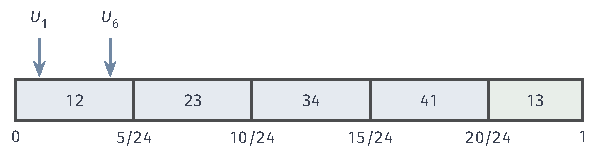
\includegraphics{figures/03-graphs/05-matrices-and-spectra/tikz/sparsification-sampling-intervals/figure.pdf}
  \caption{按各边抽样概率$p_e$切分单位区间$[0,1)$。区间内的两位数字表示边的端点。第$1$次和第$6$次的均匀随机数都落入边$12$的区间$[0,5/24)$内，因此两次增量$\frac45$均累加在边$12$上。}
  \label{fig:sparsification-sampling-intervals}
\end{BookInlineFigure}

\begin{table}[!htb]
  \centering
  \caption{四点五边图在$q=6$次抽样下的边权累加过程。}
  \label{tab:graph-resistance-sampling}
  \begin{tabular}{ccrrrrr}
    \toprule
    抽样序号 & 抽中的边 & $\widehat c_{12}$ & $\widehat c_{23}$ & $\widehat c_{34}$ & $\widehat c_{41}$ & $\widehat c_{13}$ \\
    \midrule
    1 & $12$ & $4/5$ & 0 & 0 & 0 & 0 \\
    2 & $23$ & $4/5$ & $4/5$ & 0 & 0 & 0 \\
    3 & $34$ & $4/5$ & $4/5$ & $4/5$ & 0 & 0 \\
    4 & $41$ & $4/5$ & $4/5$ & $4/5$ & $4/5$ & 0 \\
    5 & $13$ & $4/5$ & $4/5$ & $4/5$ & $4/5$ & 1 \\
    6 & $12$ & $8/5$ & $4/5$ & $4/5$ & $4/5$ & 1 \\
    \bottomrule
  \end{tabular}
\end{table}

\subsection{算法分析}
\label{sec:graph-resistance-sampling-analysis}

引理~\ref{lem:graph-resistance-sampling-moments}(1)保证了抽样图在平均意义下满足$\mathbb E[\bm L_H]=\bm L_G$；但实际算法只生成一张随机图$\mathcal H$，我们需要保证这张图以高概率\emph{同时在所有向量方向$\bm x\in\mathbb R^n$上}满足$(1-\varepsilon)\bm x^\top\bm L_G\bm x\leq\bm x^\top\bm L_H\bm x\leq(1+\varepsilon)\bm x^\top\bm L_G\bm x$。

在正交补空间$\bm 1^\perp$的能量坐标下，所有方向上的二次型能量比值都被夹在随机矩阵和$\sum_{j=1}^q\bm X_j$的最小特征值与最大特征值之间。因此，全部方向同时满足$1\pm\varepsilon$谱近似，当且仅当算子范数偏差满足$\bigl\lVert\sum_{j=1}^q\bm X_j-\bm I_{\bm 1^\perp}\bigr\rVert_2\leq\varepsilon$。下面的\term{矩阵Chernoff界}（matrix Chernoff bound）\scite{tropp2012userfriendly}专门用于控制独立随机半正定矩阵和的极端特征值偏离。

\begin{theorem}[矩阵Chernoff界的单位均值形式]
\label{thm:graph-matrix-chernoff}
设$\bm X_1,\ldots,\bm X_q$是相互独立的$d\times d$随机对称半正定矩阵，满足对每个$j$恒有$\lVert\bm X_j\rVert_2\leq r$，且期望之和为单位矩阵$\sum_{j=1}^q\mathbb E[\bm X_j]=\bm I_d$。则对任意$0<\varepsilon<1$，有
\begin{equation}
\mathbb P\!\left(
  \left\lVert\sum_{j=1}^q\bm X_j-\bm I_d\right\rVert_2>\varepsilon
\right)
\leq 2d\exp\!\left(-\frac{\varepsilon^2}{3r}\right).
\label{eq:graph-matrix-chernoff}
\end{equation}
\end{theorem}

将引理~\ref{lem:graph-resistance-sampling-moments}建立的无偏性与单次范数界$r=(n-1)/q$代入定理~\ref{thm:graph-matrix-chernoff}，立即可导出有效电阻抽样的谱稀疏化主定理。

\begin{theorem}[有效电阻抽样的谱稀疏化保证]
\label{thm:graph-resistance-sparsification}
设$\mathcal G$是含$n\geq 2$个顶点的连通正权图，给定相对误差$0<\varepsilon<1$与失败概率上限$0<\delta<1$。若按有效电阻概率$p_e=c_eR_e/(n-1)$执行算法~\ref{alg:graph-resistance-sampling}，且抽样次数$q$满足
\begin{equation}
q\geq\frac{3(n-1)}{\varepsilon^2}
         \log\frac{2(n-1)}{\delta},
\label{eq:graph-resistance-sampling-count}
\end{equation}
则输出的包含至多$\min\{m,q\}$条边的重加权子图$\mathcal H$以至少$1-\delta$的概率是$\mathcal G$的$\varepsilon$谱近似：
\[
  (1-\varepsilon)\bm L_G\preceq\bm L_H\preceq(1+\varepsilon)\bm L_G.
\]
\end{theorem}

\begin{proof}
在维数$d=n-1$的子空间$\bm 1^\perp$上考察独立随机半正定矩阵$\bm X_1,\ldots,\bm X_q$。由引理~\ref{lem:graph-resistance-sampling-moments}，有$\sum_{j=1}^q\mathbb E[\bm X_j]=\bm I_{\bm 1^\perp}$且$\lVert\bm X_j\rVert_2=(n-1)/q=r$。代入式~\eqref{eq:graph-matrix-chernoff}得
\[
\mathbb P\!\left(
  \left\lVert\sum_{j=1}^q\bm X_j-\bm I_{\bm 1^\perp}\right\rVert_2>\varepsilon
\right)
\leq 2(n-1)\exp\!\left(-\frac{q\varepsilon^2}{3(n-1)}\right).
\]
当$q$满足式~\eqref{eq:graph-resistance-sampling-count}时，右端失败概率不超过$\delta$。在概率至少为$1-\delta$的成功事件上，对任意$\bm y=\bm L_G^{1/2}\bm x\in\bm 1^\perp$都有$(1-\varepsilon)\lVert\bm y\rVert_2^2\leq\bm y^\top\bigl(\sum_{j=1}^q\bm X_j\bigr)\bm y\leq(1+\varepsilon)\lVert\bm y\rVert_2^2$，换回原坐标即得$(1-\varepsilon)\bm x^\top\bm L_G\bm x\leq\bm x^\top\bm L_H\bm x\leq(1+\varepsilon)\bm x^\top\bm L_G\bm x$。又因常向量$\bm 1$在$\bm L_G$与$\bm L_H$下的二次型均为$0$，该不等式对全体$\bm x\in\mathbb R^n$成立。
\end{proof}

若算法~\ref{alg:graph-resistance-sampling}使用的是第~\ref{sec:electrical-approximate-resistance}小节求得的近似有效电阻$\widehat R_e\in[(1-\eta)R_e,(1+\eta)R_e]$（$0\leq\eta<1$），则实际抽样概率满足$\widehat p_e\geq\frac{1-\eta}{1+\eta}p_e$，单次范数上界至多放大为$r=\frac{1+\eta}{1-\eta}\cdot\frac{n-1}{q}$。因此，将式~\eqref{eq:graph-resistance-sampling-count}中的抽样次数乘以$(1+\eta)/(1-\eta)$即可控制条件于电阻估计成功事件的抽样失败概率。当$\eta$固定且远离$1$时，这才是常数因子；若估计本身以概率至多$\delta_R$失败，则总失败概率至多为$\delta_R+\delta$。

边数为$O(n\log(n/\delta)/\varepsilon^2)$并不单独证明构造时间近线性：总成本还包含有效电阻估计、概率表预处理和抽样。采用相应的快速拉普拉斯求解器并控制求解误差，才能得到近线性的构造时间保证。

\section{稀疏图作为预条件}
\label{sec:graph-sparse-preconditioning}

拿到一张谱近似图之后，一个直接的用途是帮助求解原图上的拉普拉斯方程$\bm L_G\bm x=\bm b$。

求解的基本循环是这样的。给定当前的猜测$\bm x$，先算出它在原图上还差多少——残差$\bm r=\bm b-\bm L_G\bm x$。如果能精确解一次$\bm L_G\bm z=\bm r$，那么把$\bm z$加到$\bm x$上就直接补齐了差额。但这需要再解一次原图方程，和原问题一样难。

换一个思路：用边数少得多的近似图$\mathcal H$来求方向。也就是解$\bm L_H\bm z=\bm r$，把$\bm z$作为修正方向。这个方向不完全正确，因为$\bm L_H$和$\bm L_G$不一样。但如果两者足够接近，方向偏差不大，沿着它调整后再回到原图检查残差，几轮下来就能逼近真解。每轮用原图算残差确保终点准确，用稀疏图算方向减少计算量——这就是预条件的思路。

设原图$\mathcal G$连通，相容右端$\bm b\in\bm 1^\perp$，取$\mathcal G$的一个$\varepsilon$谱近似图$\mathcal H$（$0<\varepsilon<1$），以其拉普拉斯矩阵$\bm M=\bm L_H$作为预条件矩阵。在正交补空间$\bm 1^\perp$上，$\bm L_G$与$\bm M$均对称正定。下面的定理给出预条件算子的条件数上界以及\term{预条件共轭梯度法}（preconditioned conjugate gradient method，PCG）的收敛速度。

\begin{theorem}[谱近似预条件的条件数与收敛界]
\label{prop:graph-sparse-preconditioner}
设连通图$\mathcal G$的替代图$\mathcal H$满足$(1-\varepsilon)\bm L_G\preceq\bm M=\bm L_H\preceq(1+\varepsilon)\bm L_G$（$0<\varepsilon<1$）。在$\bm 1^\perp$上定义对称正定预条件算子$\bm A=\bm M^{-1/2}\bm L_G\bm M^{-1/2}$，则：
\begin{enumerate}
  \item 广义Rayleigh商与预条件算子$\bm A$的谱条件数满足
  \begin{equation}
  \frac{1}{1+\varepsilon}
  \leq
  \frac{\bm x^\top\bm L_G\bm x}{\bm x^\top\bm M\bm x}
  \leq
  \frac{1}{1-\varepsilon}\quad(\forall\bm x\in\bm 1^\perp\setminus\{\bm 0\}),
  \qquad
  \kappa_2(\bm A)\leq\frac{1+\varepsilon}{1-\varepsilon}.
  \label{eq:graph-sparse-preconditioned-condition}
  \end{equation}
  \item 以$\bm M$为预条件矩阵求解$\bm L_G\bm x=\bm b$（$\bm b\in\bm 1^\perp$，记零均值精确解为$\bm x_*=\bm L_G^\dagger\bm b$），预条件共轭梯度法第$k$步迭代解$\bm x^{(k)}$满足
  \begin{equation}
  \lVert\bm x^{(k)}-\bm x_*\rVert_{\bm L_G}
  \leq
  2\left(\frac{\sqrt\kappa-1}{\sqrt\kappa+1}\right)^k
  \lVert\bm x^{(0)}-\bm x_*\rVert_{\bm L_G},
  \qquad \kappa=\kappa_2(\bm A)\leq\frac{1+\varepsilon}{1-\varepsilon}.
  \label{eq:graph-sparse-preconditioned-cg-error}
  \end{equation}
\end{enumerate}
\end{theorem}

\begin{proof}
（1）对任意非零$\bm x\in\bm 1^\perp$，将$(1-\varepsilon)\bm x^\top\bm L_G\bm x\leq\bm x^\top\bm M\bm x\leq(1+\varepsilon)\bm x^\top\bm L_G\bm x$移项取倒数，即得广义Rayleigh商夹逼式：
\begin{equation}
\frac{1}{1+\varepsilon}
\leq
\frac{\bm x^\top\bm L_G\bm x}{\bm x^\top\bm M\bm x}
\leq
\frac{1}{1-\varepsilon}.
\label{eq:graph-sparse-preconditioned-rayleigh}
\end{equation}
作可逆坐标变换$\bm y=\bm M^{1/2}\bm x\in\bm 1^\perp$，则$\frac{\bm x^\top\bm L_G\bm x}{\bm x^\top\bm M\bm x}=\frac{\bm y^\top\bm A\bm y}{\bm y^\top\bm y}$正是$\bm A=\bm M^{-1/2}\bm L_G\bm M^{-1/2}$的普通Rayleigh商。因此$\lambda_{\min}(\bm A)\geq\frac{1}{1+\varepsilon}$且$\lambda_{\max}(\bm A)\leq\frac{1}{1-\varepsilon}$，两者相除即得$\kappa_2(\bm A)=\frac{\lambda_{\max}(\bm A)}{\lambda_{\min}(\bm A)}\leq\frac{1+\varepsilon}{1-\varepsilon}$。

（2）将$\bm x=\bm M^{-1/2}\bm y$代入$\bm L_G\bm x=\bm b$并左乘$\bm M^{-1/2}$，转化为等价的对称正定系统$\bm A\bm y=\bm M^{-1/2}\bm b$（精确解为$\bm y_*=\bm M^{1/2}\bm x_*$）。对任意向量$\bm e=\bm x-\bm x_*$，对应变换后误差$\bm d=\bm y-\bm y_*=\bm M^{1/2}\bm e$的$\bm A$-能量范数平方恰好等于$\bm e$的原图$\bm L_G$-能量范数平方：
\[
  \lVert\bm d\rVert_{\bm A}^2=\bm d^\top\bm A\bm d=(\bm M^{1/2}\bm e)^\top\bm M^{-1/2}\bm L_G\bm M^{-1/2}(\bm M^{1/2}\bm e)=\bm e^\top\bm L_G\bm e=\lVert\bm e\rVert_{\bm L_G}^2.
\]
直接对$\bm A\bm y=\bm M^{-1/2}\bm b$应用第~\ref{sec:electrical-numerical-solve}小节的共轭梯度误差界~\eqref{eq:electrical-cg-error}，即得式~\eqref{eq:graph-sparse-preconditioned-cg-error}。
\end{proof}

在实际执行预条件共轭梯度法时，无需显式计算平方根$\bm M^{1/2}$，而是在原坐标下每轮只做两项核心操作：先在原图$\mathcal G$上计算一次矩阵向量乘法$\bm L_G\bm p$以更新步长与残差$\bm r$，再在稀疏图$\mathcal H$上求解一次预条件方程$\bm M\bm z=\bm r$以获得修正方向$\bm z$（完整算法递推见\BookChapterRef{chap:krylov-methods}{卷二“Krylov子空间法”章}）。

若采用单点接地方式，只需在$\mathcal G$和$\mathcal H$中选取同一个接地点$q$：将接地点坐标取零的向量代入式~\eqref{eq:graph-spectral-approximation-energy}，即知两个$(n-1)\times(n-1)$约化正定矩阵$\overline{\bm L}_G$与$\overline{\bm M}=\overline{\bm L}_H$满足完全相同的谱近似界和条件数上界~\eqref{eq:graph-sparse-preconditioned-condition}。

\paragraph{一个完整的迭代例子}

用四点五边图直接看预条件后的效果。令$\mathcal G$为单位权五边图，$\mathcal H$删去对角线$13$后只保留单位权四环。两图在$\bm 1^\perp$上有三个独立的零和方向。

先看$\bm u=(1,0,-1,0)^\top$。对角边两端之差为$2$，贡献能量$4$，加上四条环边各$1$，原图能量为$8$。四环没有对角边，能量只有$4$。广义Rayleigh商$8/4=2$。

再看与$\bm u$正交的零和方向，比如$\bm v=(0,1,0,-1)^\top$。此时对角边两端同值$0$，不贡献能量。两图能量都是$4$（该向量长度平方为$2$、特征值为$2$），商为$1$。

还有一个方向（如$(1,-1,1,-1)^\top/2$归一化），也可核对对角边上差为零。因此四环$\bm M$在$\bm u$方向的特征值是$2$，添对角边后$\bm L_G$在同方向变为$4$，而其余两个方向上两图一样。预条件矩阵$\bm A$的三个特征值为$1,1,2$。通用界$\varepsilon=1/2$给出条件数上界$(1+1/2)/(1-1/2)=3$，覆盖了实际条件数$2$。

用同一例子走一轮迭代。设右端$\bm b=\bm u+\bm v$，初值为零。第一次残差就是$\bm b$。在四环上解$\bm M\bm z=\bm b$，得到$\bm z=(\bm u+\bm v)/2$。

沿$\bm z$更新时，步长由原图决定。因为$\bm u,\bm v$正交且长度平方都是$2$，
\[
\bm b^\top\bm z=2,
\qquad
\bm z^\top\bm L_G\bm z=3.
\]
步长为$2/3$。更新后$\bm x^{(1)}=(\bm u+\bm v)/3$。残差为
\[
\bm b-\bm L_G\bm x^{(1)}
=\frac{-\bm u+\bm v}{3}.
\]
这个残差还含两个方向，下一轮用它继续修正。图~\ref{fig:sparsification-preconditioner-step}把两张图的分工画了出来：四环给出修正方向，原图决定步长和检验残差。

\begin{BookInlineFigure}
  \centering
  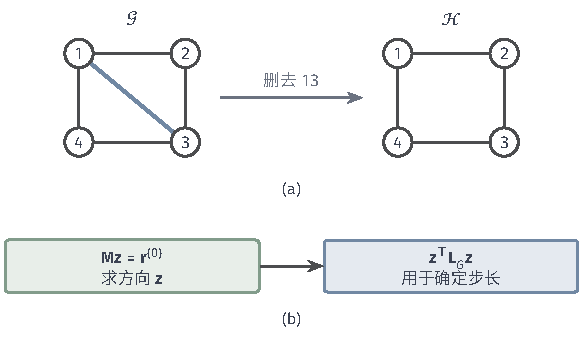
\includegraphics{figures/03-graphs/05-matrices-and-spectra/tikz/sparsification-preconditioner-step/figure.pdf}
  \caption{四点五边图的预条件迭代。（a）原图$\mathcal G$和删去对角边后的四环$\mathcal H$。（b）第一轮用$\mathcal H$的拉普拉斯求方向，用$\mathcal G$的拉普拉斯计算步长和残差。}
  \label{fig:sparsification-preconditioner-step}
\end{BookInlineFigure}

\paragraph{实际代价}

总代价包含三部分：构造稀疏图并准备它的求解器（一次性），每轮在原图上做一次矩阵乘向量（$O(m+n)$），以及每轮在稀疏图上解方程。同一图有多个右端时，可以共享近似图及其分解，把准备成本分摊给多次求解。

稀疏图虽然边少，但直接分解时仍可能产生填充——是否值得要同时比较每轮代价和所需迭代次数。若每轮在近似图上只做有限次内迭代而非精确求解，需要另行控制求解误差，不能直接套用式~\eqref{eq:graph-sparse-preconditioned-cg-error}中精确预条件的结论。

\section{本章小结}
\label{sec:graph-sparsification-summary}

本章研究如何用边数少得多的带权图代替原图，同时近似保持计算结果。

若替代图只用于评价分组，只需保持割权——单点割给出加权度，加权度相加给出体积，割权与体积共同决定导通率和NCut。若还要求特征值、有效电阻或方程解，就需要保持所有实值顶点赋值上的能量，即谱近似。同一个三角形的例子说明，割近似不自动蕴含谱近似：边权的增减可能集中在差异大或差异小的方向上，只看跨边总权无法发现。

每条边在随机生成树中出现的概率是$c_eR_e$，这个乘积由电导和有效电阻共同决定。桥必定出现在每棵树中，团内边只出现在一部分树中。把这些概率除以Foster总和$n-1$，得到加起来等于一的抽样分布。每次抽到一条边后按概率的倒数补偿权重，使平均矩阵恰好等于原矩阵。有效电阻抽样的关键性质是：不论抽到哪条边，单次贡献在标准化坐标中的范数都是同一个值$(n-1)/q$，它均衡了所有边在最坏方向上的波动。矩阵Chernoff界把这个单次上界转为"所有方向同时满足误差"的概率保证。

用稀疏图作预条件时，每轮在原图上算残差，在稀疏图上根据残差求修正方向。两图能量之比越接近一，换坐标后的矩阵越接近恒等算子，条件数越小，所需迭代次数越少。实际节省多少工作，还要加上构造稀疏图和准备其求解器的开销。

